\begin{frame}{Результати роботи}
	\framesubtitle{Інтегральне рівняння для першого моменту}
	В роботі було виведене інтегральне рівняння зі зсувом для математичного сподівання $m_{p}(x)$ максимальної кількості автомобілів на паркінгу довжини $x$.
	\begin{thm}
		У випадку розташування автомобілів за сумішшю рівномірного та детермінованого розподілів \eqref{eq:general_dist} виконується наступне співвідношення:
        \begin{equation}
		m_{p}(x + 1) = 1 + p m_{p}(x) + \frac{2(1-p)}{x} \int\limits_0^{x} m_{p}(t) dt,\quad \forall x > 0
        \end{equation}
	\end{thm}
\end{frame}

\begin{frame}{Результати роботи}
	\framesubtitle{Асимптотична поведінка першого моменту}
	Було доведено асимптотичну формулу для $m_{p}(x)$ при $x \rightarrow \infty$.
	\begin{thm}
		Перший момент випадкової величини $N_{p}(x)$ прямує до лінійної функції від довжини парковки $x$ з швидкістю, вищою за поліноміальну:
		\begin{gather}
		m_{p}(x) = C_{p} x - \frac{1 - C_{p}}{1-p} + \mathcal{O}(x^{-n}) \quad \forall n \in \mathbb{N}, \\
		\text{де }C_{p} = \frac{1}{1-p}  \int\limits_0^\infty \exp\left( -2\int\limits_0^s \frac{e^{\tau} - 1}{\tau(e^\tau - p)}\,d\tau\right)\,ds \label{eq:c_p_integral}.
		\end{gather}
	\end{thm}
	\note{На основі інтегрального рівняння було отримано асимптотику математичного сподівання $m_p(x)$ максимальної кількості автомобілів на паркінгу довжини $x$ при $x \rightarrow \infty$.}
\end{frame}

\begin{frame}{Результати роботи}
\framesubtitle{Закон великих чисел для рівня заповненості}
Було показано, що має місце закон великих чисел для рівня заповненості вихідного відрізку $\frac{N_{p}(x)}{x}$. Тобто, при достатньо великих розмірах парковки можна практично вважати, що $N_{p}(x)=C_{p}x$.
\begin{thm}
	У випадку розташування автомобілів за сумішшю рівномірного та детермінованого розподілів \eqref{eq:general_dist} відношення $\frac{N_{p}(x)}{x}$ стохастично прямує до $C_{p}$ при $x \rightarrow \infty$.
	\begin{equation}
	\Prob{\left|\frac{N_{p}(x)}{x} - C_{p}\right| > \varepsilon} \rightarrow 0, \quad x \rightarrow \infty.
	\end{equation}
\end{thm}
\note{}
\end{frame}

\begin{frame}{Результати роботи}
	\framesubtitle{Оцінка константи $C_{p}$ методом чисельного інтегрування}
	\begin{columns}
		\begin{column}{0.5\textwidth}
			Приблизне значення сталої $C_{p}$ можна визначити з формули \eqref{eq:c_p_integral} за допомогою чисельної аппроксимації.
		\end{column}
		\begin{column}{0.5\textwidth}
			\begin{figure}
				\centering
				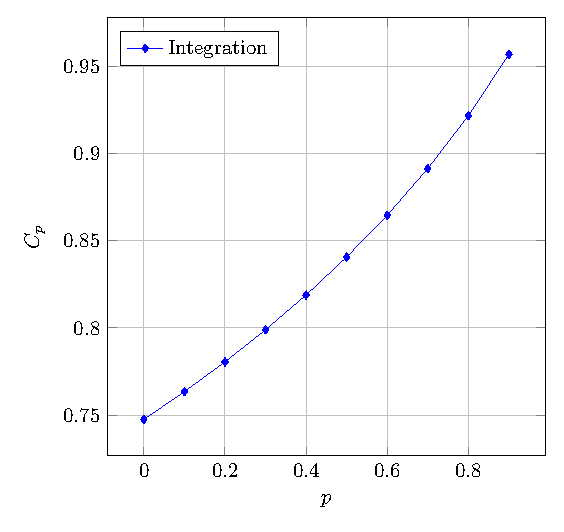
\includegraphics[scale=0.5]{im/integ_cp}
			\end{figure}
		\end{column}
	\end{columns}
\end{frame}

\begin{frame}{Результати роботи}
\framesubtitle{Оцінка константи $C_{p}$ методом імітаційного моделювання}
\begin{columns}
	\begin{column}{0.5\textwidth}
		Приблизне значення сталої $C_{p}$ можна визначити методом Монте-Карло, усереднюючи по великій кількості експериментів. В межах одного експерименту проводиться імітаційне моделювання процесу паркування з досить великим розміром парковки.
	\end{column}
	\begin{column}{0.5\textwidth}
		\begin{figure}
			\centering
			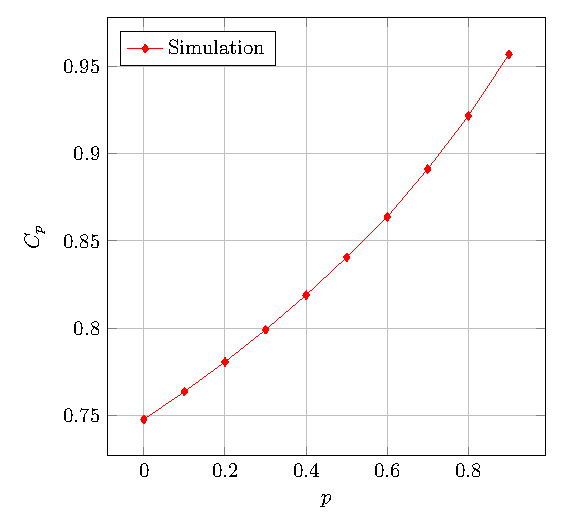
\includegraphics[scale=0.5]{im/simul_cp}
		\end{figure}
	\end{column}
\end{columns}
\end{frame}

\begin{frame}{Результати роботи}
\framesubtitle{Порівняння значень $C_{p}$, отриманих двома способами}
\begin{figure}
	\centering
	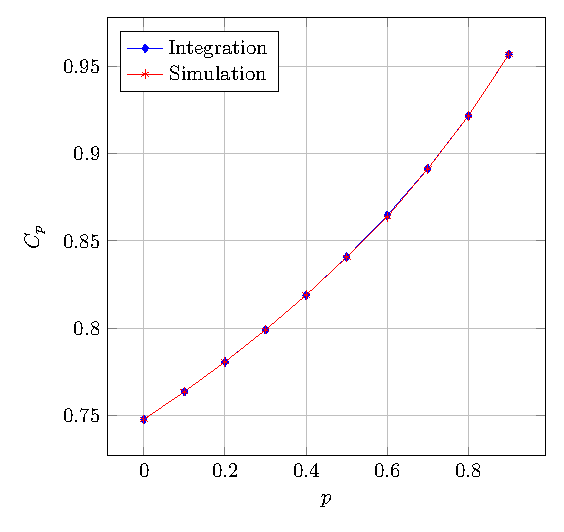
\includegraphics[scale=0.8]{im/composite_cp}
\end{figure}
\end{frame}


